\documentclass[]{elsarticle} %review=doublespace preprint=single 5p=2 column
%%% Begin My package additions %%%%%%%%%%%%%%%%%%%
\usepackage[hyphens]{url}
\usepackage{lineno} % add
\providecommand{\tightlist}{%
  \setlength{\itemsep}{0pt}\setlength{\parskip}{0pt}}

\bibliographystyle{elsarticle-harv}
\biboptions{sort&compress} % For natbib
\usepackage{graphicx}
\usepackage{booktabs} % book-quality tables
%% Redefines the elsarticle footer
%\makeatletter
%\def\ps@pprintTitle{%
% \let\@oddhead\@empty
% \let\@evenhead\@empty
% \def\@oddfoot{\it \hfill\today}%
% \let\@evenfoot\@oddfoot}
%\makeatother

% A modified page layout
\textwidth 6.75in
\oddsidemargin -0.15in
\evensidemargin -0.15in
\textheight 9in
\topmargin -0.5in
%%%%%%%%%%%%%%%% end my additions to header

\usepackage[T1]{fontenc}
\usepackage{lmodern}
\usepackage{amssymb,amsmath}
\usepackage{ifxetex,ifluatex}
\usepackage{fixltx2e} % provides \textsubscript
% use upquote if available, for straight quotes in verbatim environments
\IfFileExists{upquote.sty}{\usepackage{upquote}}{}
\ifnum 0\ifxetex 1\fi\ifluatex 1\fi=0 % if pdftex
  \usepackage[utf8]{inputenc}
\else % if luatex or xelatex
  \usepackage{fontspec}
  \ifxetex
    \usepackage{xltxtra,xunicode}
  \fi
  \defaultfontfeatures{Mapping=tex-text,Scale=MatchLowercase}
  \newcommand{\euro}{€}
\fi
% use microtype if available
\IfFileExists{microtype.sty}{\usepackage{microtype}}{}
\usepackage{longtable}
\usepackage{graphicx}
% We will generate all images so they have a width \maxwidth. This means
% that they will get their normal width if they fit onto the page, but
% are scaled down if they would overflow the margins.
\makeatletter
\def\maxwidth{\ifdim\Gin@nat@width>\linewidth\linewidth
\else\Gin@nat@width\fi}
\makeatother
\let\Oldincludegraphics\includegraphics
\renewcommand{\includegraphics}[1]{\Oldincludegraphics[width=\maxwidth]{#1}}
\ifxetex
  \usepackage[setpagesize=false, % page size defined by xetex
              unicode=false, % unicode breaks when used with xetex
              xetex]{hyperref}
\else
  \usepackage[unicode=true]{hyperref}
\fi
\hypersetup{breaklinks=true,
            bookmarks=true,
            pdfauthor={},
            pdftitle={Draft paper on collecting vegetation indices using citizen science},
            colorlinks=true,
            urlcolor=blue,
            linkcolor=magenta,
            pdfborder={0 0 0}}
\urlstyle{same}  % don't use monospace font for urls
\setlength{\parindent}{0pt}
\setlength{\parskip}{6pt plus 2pt minus 1pt}
\setlength{\emergencystretch}{3em}  % prevent overfull lines
\setcounter{secnumdepth}{0}
% Pandoc toggle for numbering sections (defaults to be off)
\setcounter{secnumdepth}{0}
% Pandoc header


\usepackage[nomarkers]{endfloat}

\begin{document}
\begin{frontmatter}

  \title{Draft paper on collecting vegetation indices using citizen science}
    \author[a]{R. Willem Vervoort\corref{c1}}
   \ead{willem.vervoort@sydney.edu.au} 
   \cortext[c1]{Corresponding Author}
    \author[b]{Dasapta Erwin Irawan}
   \ead{dasaptaerwin@gmail.com} 
  
    \author[c]{Gene Melzack}
   \ead{gene.melzack@sydney.edu.au} 
  
      \address[a]{The University of Sydney, Department, Street, City, State, Zip}
    \address[b]{ITB, Department, Street, City, State, Zip}
    \address[c]{The University of Sydney Library, Department, Street, City, State, Zip}
  
  \begin{abstract}
  Understanding the spatial and temporal variation in primary production
  can identify variation in ecological response related to climate and
  landscape. With mobile phone cameras now easily available, this opens an
  opportunity to use citizen science to record primary production from
  vegetation images.
  
  The objective of this study is to demonstrate how mobile phone images
  can be quickly analysed for primary production and can give inside in
  spatial variation of ecological response.
  
  Participants in an open data workshop took mobile phone imagery of local
  vegetation and the resulting images were stored in an open data project
  folder. The images were analysed and used to quantify vegetation indices
  of primary production, which was plotted in space.
  
  The results indicate a wide variation of vegetation indices, even across
  a small area. The process of taking images, uploading, sharing and
  analysis was rapid using basic open data science tools.
  
  Mobile phones can be used by inexperienced operators to quickly map
  vegetation indices in an area.
  \end{abstract}
  
 \end{frontmatter}

\section{Introduction}\label{introduction}

The evolving nature of science publishing has lead to a strong growth in
open science (D. Irawan et al. 2017) and citizen science efforts
(Dickinson, Zuckerberg, and Bonter 2010). With this comes a need to
create an understanding of open science and the potentials of open
science for researchers in different fields. To assist with this a
workshop was organised at Institut Teknologi Bandung (ITB) in
collaboration with the University of Sydney (USYD) (D. E. Irawan,
Vervoort, and Melzack 2018) to demonstrate different aspect of open
science and open science publishing.

During the workshop, an example dataset was used based on older research
(R. W. Vervoort and Annen 2006). During the workshop , participants were
introduced in components, such as defining metadata, creating spatial
and netcdfdata, and recording workflows. During the last day of the
workshop, new data were generated using vegetation photographs from
mobile phones in the field to allow the participants to practice skills
learned.

There is considerable interest globally in remotely mapping vegetation
due to its strong relationship with ecosystem health and variation in
drivers of vegetation productivity (Huete et al. 2011; Rohde, Froend,
and Howard 2017). Ratios of colour bands in vegetation photographs have
been shown to be highly correlated to gross primary production (Moore et
al. 2017), and this therefore creates opportunities for rapid local
mapping of vegetation growth and condition.

The objective of this paper is to demonstrate how the collected data can
be easily summarised and a draft paper written using Rmarkdown and the
package \texttt{rticles}.

\section{Methods}\label{methods}

\subsection{Data collection}\label{data-collection}

Using mobile phones, data were collected by the participants at several
locations on a field site in Bandung, by simply taking photos of the
existing vegetation. These photos were downloaded from the phones and
collected in a data folder on
\href{https://drive.google.com/drive/folders/1jgMlC3NbL_7dFVb29AjNflgxqPj6LLMf?usp=sharing}{the
project Google drive storage}.

\subsection{Data processing}\label{data-processing}

Metadata were extracted from the photos using the exif program, using
the R package \texttt{exifr}. This focussed specifically on the latitude
and longitude information as this could be used for further mapping.
However, other metadata, such as cameratype and time of collection, can
also easily be extracted.

Using the package \texttt{imager} in R, the image colour bands were
extracted from the photos and following Moore et al. (2017) the ratio
(GCC) of the green band (G) over the sum of the red (R) and blue (B)
bands was calculated:

/begin\{equation\} GCC = /frac\{G\}\{(R + B)\} /label\{eqn:model\}
/end\{equation\}

\section{Results}\label{results}

Using Rmarkdown, we can run all the analysis in the background and not
show this in the paper. However the workflow is still recorded in the
code blocks in the ``Rmd'' file that generates the document. This means
the analysis is still repeatable even though this is not directly
visible in the article.

As a first result we can show a table of the result with the associated
latitudes and longitudes. This can easily be done using \texttt{pander}
which creates nice tables. This shows that there is quite a range of
variability in the data.

\begin{longtable}[]{@{}ccc@{}}
\caption{Table 1 Overview of first 10 collected data and GCC
values}\tabularnewline
\toprule
\begin{minipage}[b]{0.14\columnwidth}\centering\strut
Latitude\strut
\end{minipage} & \begin{minipage}[b]{0.15\columnwidth}\centering\strut
Longitude\strut
\end{minipage} & \begin{minipage}[b]{0.08\columnwidth}\centering\strut
GCC\strut
\end{minipage}\tabularnewline
\midrule
\endfirsthead
\toprule
\begin{minipage}[b]{0.14\columnwidth}\centering\strut
Latitude\strut
\end{minipage} & \begin{minipage}[b]{0.15\columnwidth}\centering\strut
Longitude\strut
\end{minipage} & \begin{minipage}[b]{0.08\columnwidth}\centering\strut
GCC\strut
\end{minipage}\tabularnewline
\midrule
\endhead
\begin{minipage}[t]{0.14\columnwidth}\centering\strut
NA\strut
\end{minipage} & \begin{minipage}[t]{0.15\columnwidth}\centering\strut
NA\strut
\end{minipage} & \begin{minipage}[t]{0.08\columnwidth}\centering\strut
0.58\strut
\end{minipage}\tabularnewline
\begin{minipage}[t]{0.14\columnwidth}\centering\strut
NA\strut
\end{minipage} & \begin{minipage}[t]{0.15\columnwidth}\centering\strut
NA\strut
\end{minipage} & \begin{minipage}[t]{0.08\columnwidth}\centering\strut
0.6\strut
\end{minipage}\tabularnewline
\begin{minipage}[t]{0.14\columnwidth}\centering\strut
-6.888\strut
\end{minipage} & \begin{minipage}[t]{0.15\columnwidth}\centering\strut
107.6\strut
\end{minipage} & \begin{minipage}[t]{0.08\columnwidth}\centering\strut
0.53\strut
\end{minipage}\tabularnewline
\begin{minipage}[t]{0.14\columnwidth}\centering\strut
-6.888\strut
\end{minipage} & \begin{minipage}[t]{0.15\columnwidth}\centering\strut
107.6\strut
\end{minipage} & \begin{minipage}[t]{0.08\columnwidth}\centering\strut
0.59\strut
\end{minipage}\tabularnewline
\begin{minipage}[t]{0.14\columnwidth}\centering\strut
-6.888\strut
\end{minipage} & \begin{minipage}[t]{0.15\columnwidth}\centering\strut
107.6\strut
\end{minipage} & \begin{minipage}[t]{0.08\columnwidth}\centering\strut
0.53\strut
\end{minipage}\tabularnewline
\begin{minipage}[t]{0.14\columnwidth}\centering\strut
-6.888\strut
\end{minipage} & \begin{minipage}[t]{0.15\columnwidth}\centering\strut
107.6\strut
\end{minipage} & \begin{minipage}[t]{0.08\columnwidth}\centering\strut
0.53\strut
\end{minipage}\tabularnewline
\begin{minipage}[t]{0.14\columnwidth}\centering\strut
-6.888\strut
\end{minipage} & \begin{minipage}[t]{0.15\columnwidth}\centering\strut
107.6\strut
\end{minipage} & \begin{minipage}[t]{0.08\columnwidth}\centering\strut
0.53\strut
\end{minipage}\tabularnewline
\begin{minipage}[t]{0.14\columnwidth}\centering\strut
-6.888\strut
\end{minipage} & \begin{minipage}[t]{0.15\columnwidth}\centering\strut
107.6\strut
\end{minipage} & \begin{minipage}[t]{0.08\columnwidth}\centering\strut
0.53\strut
\end{minipage}\tabularnewline
\begin{minipage}[t]{0.14\columnwidth}\centering\strut
-6.888\strut
\end{minipage} & \begin{minipage}[t]{0.15\columnwidth}\centering\strut
107.6\strut
\end{minipage} & \begin{minipage}[t]{0.08\columnwidth}\centering\strut
0.56\strut
\end{minipage}\tabularnewline
\begin{minipage}[t]{0.14\columnwidth}\centering\strut
-6.888\strut
\end{minipage} & \begin{minipage}[t]{0.15\columnwidth}\centering\strut
107.6\strut
\end{minipage} & \begin{minipage}[t]{0.08\columnwidth}\centering\strut
0.51\strut
\end{minipage}\tabularnewline
\bottomrule
\end{longtable}

\begin{verbatim}
## Warning: Removed 2 rows containing missing values (geom_point).
\end{verbatim}

\begin{figure}
\centering
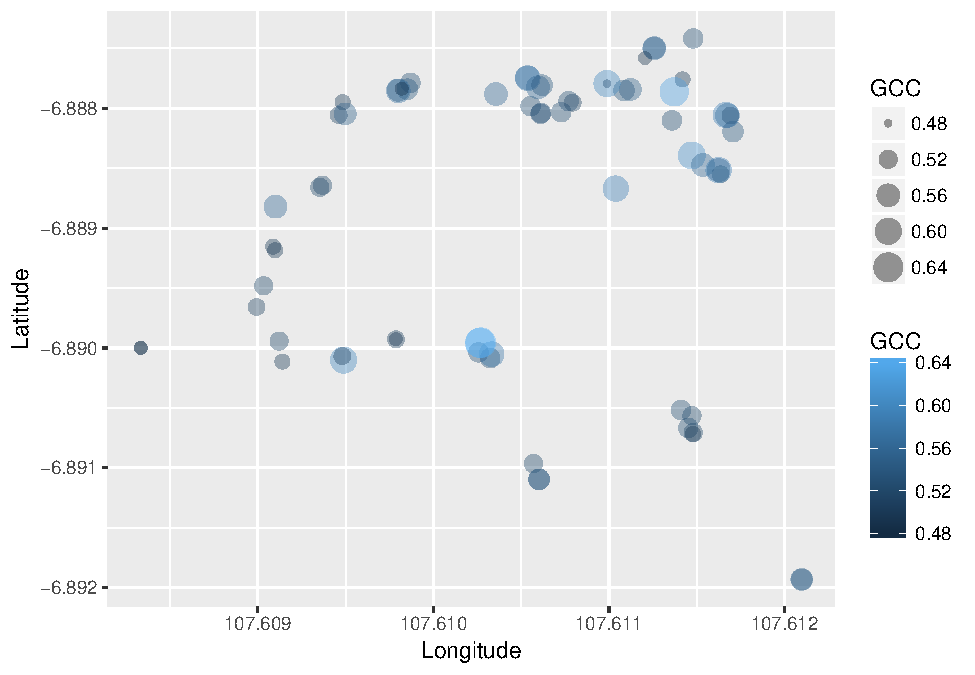
\includegraphics{DraftPaper_GCC_CitizenScience_files/figure-latex/plot_data-1.pdf}
\caption{Plot of the collected data by latitude and longitude}
\end{figure}

From the plot we can see that there are two points at one location, and
several points at a second locations. Overall the variation in GCC is
between 0.5 and 0.7. Some of the points are so close together that they
are simply overlapping.

\section{Discussion and conclusions}\label{discussion-and-conclusions}

While there are many different ways to publish research. Open Science
offers new opportunities to make data and research available to the
wider public. Rmarkdown in combination with the package \texttt{rticles}
allows for efficient recording of workflows and paper writing.

This paper has demonstrated that using existing tools it is fairly
simple to produce a draft paper that includes the overall workflow
within the document.

It also demonstrates that using mobile phone photography it is easy to
collect a large amount of data using inexperienced (citizen science)
type data collection and to quickly summarize this data.

\section*{References}\label{references}
\addcontentsline{toc}{section}{References}

\hypertarget{refs}{}
\hypertarget{ref-dickinson_citizen_2010}{}
Dickinson, Janis L., Benjamin Zuckerberg, and David N. Bonter. 2010.
``Citizen Science as an Ecological Research Tool: Challenges and
Benefits.'' \emph{Annual Review of Ecology, Evolution, and Systematics}
41 (1): 149--72.
doi:\href{https://doi.org/10.1146/annurev-ecolsys-102209-144636}{10.1146/annurev-ecolsys-102209-144636}.

\hypertarget{ref-huete_modis_2011}{}
Huete, Alfredo, Kamel Didan, Willem van Leeuwen, Tomoaki Miura, and Ed
Glenn. 2011. ``MODIS Vegetation Indices.'' In \emph{Land Remote Sensing
and Global Environmental Change: NASA's Earth Observing System and the
Science of ASTER and MODIS}, edited by Bhaskar Ramachandran, Christopher
O. Justice, and Michael J. Abrams, 579--602. New York, NY: Springer New
York. \url{https://doi.org/10.1007/978-1-4419-6749-7_26}.

\hypertarget{ref-irawan_workshop_2018}{}
Irawan, Dasapta E, Rutger W Vervoort, and Gene Melzack. 2018. ``Open
Data Workshop Sseac Usyd - Itb.'' OSF.io. \url{https://OSF.IO/S76GU/}.

\hypertarget{ref-irawan_review_2017}{}
Irawan, Dasapta, Cut Novianti Rachmi, Mochammad Multazam, Hendy Irawan,
Juneman Abraham, kustiati, KeuKeu Kaniawati Rosada, et al. 2017. ``A
Review on the Implementation of Open Science in Indonesia.'' OSF.io.
\url{https://osf.io/preprints/inarxiv/7r8jn/}.

\hypertarget{ref-moore_treegrass_2017}{}
Moore, C. E., J. Beringer, B. Evans, L. B. Hutley, and N. J. Tapper.
2017. ``Tree--grass Phenology Information Improves Light Use Efficiency
Modelling of Gross Primary Productivity for an
Australian\textbackslash{}hack\textbackslash{}newline Tropical
Savanna.'' \emph{Biogeosciences} 14 (1): 111--29.
doi:\href{https://doi.org/10.5194/bg-14-111-2017}{10.5194/bg-14-111-2017}.

\hypertarget{ref-rohde_global_2017}{}
Rohde, Melissa M., Ray Froend, and Jeanette Howard. 2017. ``A Global
Synthesis of Managing Groundwater Dependent Ecosystems Under Sustainable
Groundwater Policy.'' \emph{Groundwater} 55 (3): 293--301.
doi:\href{https://doi.org/10.1111/gwat.12511}{10.1111/gwat.12511}.

\hypertarget{ref-vervoort_palaeochannels_2006}{}
Vervoort, R. W., and Y. L. Annen. 2006. ``Palaeochannels in Northern New
South Wales: Inversion of Electromagnetic Induction Data to Infer
Hydrologically Relevant Stratigraphy.'' \emph{Soil Research} 44 (1):
35--45. \url{https://doi.org/10.1071/SR05037}.

\end{document}


